\documentclass[12pt, a4paper]{article}
\usepackage[utf8]{inputenc}
\usepackage[english]{babel}
\usepackage{fancyhdr}
\usepackage{datetime}
\usepackage{hyperref}
\usepackage{longtable}
\usepackage{graphicx}
\usepackage{listings}
\usepackage{xcolor}
\usepackage{amsfonts}
\usepackage{amsmath}
\lstset { %
    language=C++,
    backgroundcolor=\color{black!5}, % set backgroundcolor
    basicstyle=\footnotesize,% basic font setting
    keywordstyle=\color{blue}\ttfamily,
    stringstyle=\color{red}\ttfamily,
    commentstyle=\color{green}\ttfamily,
    morecomment=[l][\color{magenta}]{\#}
}
\usepackage[font=small,labelfont=bf]{caption}
\hypersetup{
    colorlinks,
    citecolor=black,
    filecolor=black,
    linkcolor=black,
    urlcolor=black
}

\def\labelitemi{--}
\setcounter{tocdepth}{3}
\pagestyle{fancy}
\fancyhf{}
\renewcommand{\headrulewidth}{1pt}
\renewcommand{\footrulewidth}{1pt}
\rhead{\leftmark}
\rfoot{Page \thepage}

\begin{document}

\begin{titlepage}

    \newcommand{\HRule}{\rule{\linewidth}{0.5mm}} % Defines a new command for the horizontal lines, change thickness here
    
    \center % Center everything on the page
     
    %----------------------------------------------------------------------------------------
    %	HEADING SECTIONS
    %----------------------------------------------------------------------------------------
    
    \textsc{\LARGE Università Degli Studi Di Milano}\\[1.5cm] % Name of your university/college
    \textsc{\Large Real-Time Graphics Programming}\\[0.5cm] % Major heading such as course name
    %\textsc{\large Assignment 1}\\[0.5cm] % Minor heading such as course title
    
    %----------------------------------------------------------------------------------------
    %	TITLE SECTION
    %----------------------------------------------------------------------------------------
    
    \HRule \\[0.4cm]
    { \huge \bfseries Real-time autostereogram rendering pipeline }\\[0.4cm] % Title of your document
    \HRule \\[1.5cm]
     
    %----------------------------------------------------------------------------------------
    %	AUTHOR SECTION
    %----------------------------------------------------------------------------------------
    
    \begin{minipage}{0.4\textwidth}
    \begin{flushleft} \large
    \emph{Author:}\\
    Giovanni \textsc{Cocco} \\
    \end{flushleft}
    \end{minipage}
    ~
    \begin{minipage}{0.4\textwidth}
    \begin{flushright} \large
    \emph{Academic year:} \\
    2022-2023\\
    \end{flushright}
    \end{minipage}\\[2cm]
    
    % If you don't want a supervisor, uncomment the two lines below and remove the section above
    %\Large \emph{Author:}\\
    %John \textsc{Smith}\\[3cm] % Your name
    
    %----------------------------------------------------------------------------------------
    %	DATE SECTION
    %----------------------------------------------------------------------------------------
    
    {\large \today}\\[4cm] % Date, change the \today to a set date if you want to be precise
    
    %----------------------------------------------------------------------------------------
    %	LOGO SECTION
    %----------------------------------------------------------------------------------------
    
    
\includegraphics[width=130px, keepaspectratio]{img/unimi.png}\\[1cm] % Include a department/university logo - this will require the graphicx package
     
    %----------------------------------------------------------------------------------------
    
    \vfill % Fill the rest of the page with whitespace
    
    \end{titlepage}

\clearpage
\tableofcontents{}
\listoffigures
\listoftables
\lstlistoflistings
\clearpage

\section{Abstract}
In this document we discuss the algorithms, the choices and the implementation details of a real-time autostereogram rendering pipeline built with OpenGL 4.3.\\\\
The pipeline presented allow the rendering of autostereograms starting from a depth buffer that is always produces
as a result on all classical rasterization rendering algorithms. More elaborated effect can be achieved if we supply as input also the color buffer and 
the normal buffer.\\\\
We will first briefly explain what an autostereogram is and how it works from a psychological point of view. We will then discuss a general algorithm to create them.
We will then discuss the implementation detail of the project.\\\\
It should be noted that the input needed for the autostereogram generation algorithm are produced as a result of most real-time rendering pipeline and this 
mean that is possible to apply this technique to an already existent rendering pipeline.\\\\
For this project we made a simple rendering pipeline using Blinn-Phong illumination model, as we will see more sophisticated model give little gain in 
the final result.\\\\
The project also implements blend skinning for skeletal animation, we will discuss the implementation and the difference between linear blend skinning and
dual quaternion skinning.\\\\
We will see how the performance of this pipeline can be totally in the frame budget on most GPU buy may suffer on old laptop one while still
providing 60 frames per second.

\clearpage
\section{Autostereogram}
\subsection{What is an autostereogram}
A stereogram is a 2D image that creates the optical illusion of a 3D scene\footnote{https://en.wikipedia.org/wiki/Autostereogram}. Autostereograms are a particular kind of stereograms
that create this illusion without requiring any additional equipment.\\\\
Our brain is able to perceive depth because each eye receives a different image because they are in slightly different positions on one's head.
We can exploit this behavior by producing one image with repeating patter causing and object to be in the right position from the point of view of each eye
if the eye separation of the subject is the correct one.\\\\
Note that it might take some practice before being able to control the eye separation and be able to see
the optical illusion. For more information on some viewing technique one may take a look at: \url{https://www.hidden-3d.com/how_to_view_stereogram.php}.\\\\
\begin{center}
    \centering
    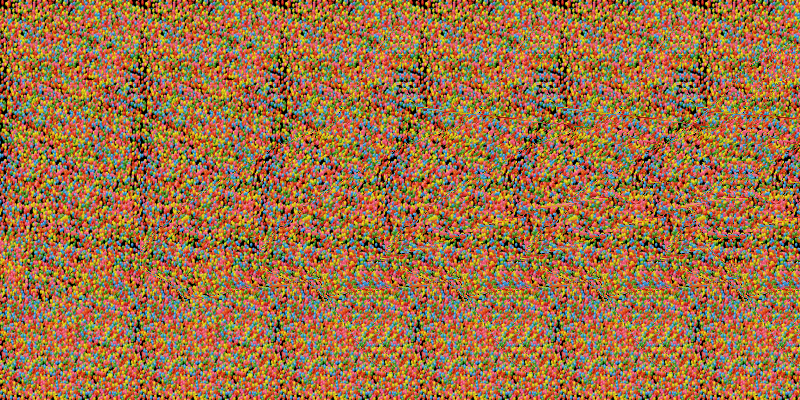
\includegraphics[width=1.0\textwidth]{img/shark.png}
    \captionof{figure}{Autostereogram of a shark}
\end{center}
\clearpage
\subsection{Autostereogram rendering algorithm}
To render an autostereogram we need first to understand the underling geometry.\\
\begin{center}
    \centering
    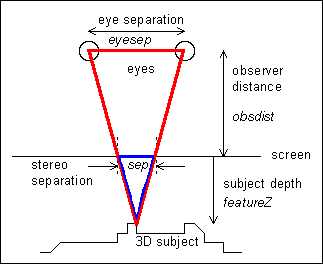
\includegraphics[width=0.7\textwidth]{img/geometry.png}
    \captionof{figure}{The geometry of an autostereogram}
\end{center}
If the two points where the line of sight intercept the screen have the same color the depth of the 3D
subject will be perceived.\\\\
As we can see from the figure the two highlighted triangles have the same angles and as such they are similar.
This means they are proportional, and so we can calculate the separation with the following equation.
\[
sep = \frac{eyesep \cdot featureZ}{featureZ + obsdist}
\]
The general method to create an autostereogram is the following\footnote{http://www.techmind.org/stereo/stech.html}:
\begin{itemize}
    \item Create a depth map of the scene.
    \item For each horizontal line, moving from left to right, and for each point of the depth map link together all the pixel that will have the same color.
    \item Assign to each point a random color making sure the linked one will have the same.
\end{itemize}

\subsection{Advanced effects}
The choice of which color assign to a pixel allow for different effect.\\\\
It is possible to use a completely random color, but is also possible use a texture pattern that will be repeated horizontally.\\\\
It is also possible to highlight the edge of the objects or using a color based on the real object color.
\begin{center}
    \centering
    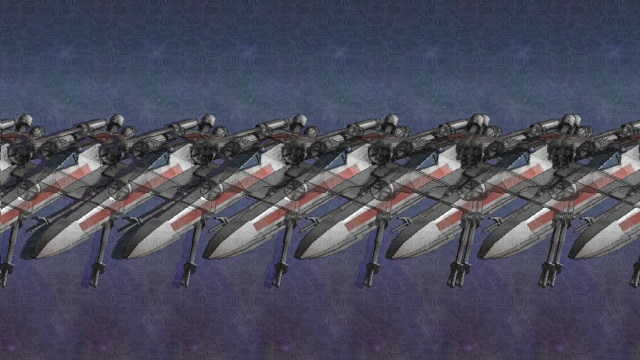
\includegraphics[width=1.0\textwidth]{img/ship.png}
    \captionof{figure}{Autostereogram where object color are used}
\end{center}
As one may expect this means objects will bleed horizontally to other pixels in a repeating fashion.
\section{Scene management}
\subsection{Handle multiple scenes}
The project requires different scenes to be loaded when selected from the GUI.\\\\
To achieve this the class \textbf{SceneManager} is responsible for loading the correct scene and unloading the old one
freeing any no longed used resources.\\\\
The \textbf{SceneManager} class hold a polymorphic pointer to a class \textbf{Scene}, when asked to load a new one
the current one is deleted and the old one is instanced creating a subclass of type \textbf{Scene}.\\\\
This mean there is a subclass of \textbf{Scene} for every scene in the project. This method in general does not
scale well, but for a project of this scale loading a scene specification from an asset file was considered overengineering.
It should be noted that if the scene was loaded from a file we could not use the polymorphic nature of the class
\textbf{Scene} to override its method \textbf{Update}. In this situation we would be required to support scripting in the
scene with something like Lua, again this was considered overengineer.\\\\
The constructor of \textbf{Scene} will load the required assets as we will discuss later. This requires up to 40MB of 
data to be loaded from the disk on demand. As this require quite some time the class \textbf{SceneManager} also
hold an instance to an object of type \textbf{LoadingScreen} that will create a simple loading screen before calling
the \textbf{Scene} constructor.
\begin{center}
    \centering
    
\includegraphics[width=1.0\textwidth]{img/loading.png}
    \captionof{figure}{Loading screen}
\end{center}
The \textbf{LoadingScreen} constructor will create the shader, the quad and the texture needed for the loading screen
rendering.\\\\
The quad is simply a square with x, y coordinate with values in -1, 1. To ensure the loading screen will be rendered correctly
in any aspect rateo the inverse of the rateo is passed to the vertex shader as a uniform called \textbf{rateo}.\\\\
The vertex shader will draw the quad as high as the screen and center horizontally.
\begin{lstlisting}[caption={Loading screen vertex shader},captionpos=b]
#version 430 core
layout (location = 0) in vec3 position;
uniform float rateo;
    
out vec2 uv;
void main() {
    uv = vec2(0.5)+position.xy*0.5;
    vec4 pos = vec4(position, 1.0);
    pos.x *= rateo;
    uv.y = -uv.y;
    gl_Position = pos;
}
\end{lstlisting}
To hide the missing part on right and left
the buffer was cleared with \textbf{glClear} with the clear color set as the loading screen image background color.\\\\
The \textbf{SceneManager} also forward the call to the method process to the current loaded scene to allow the scene
to be updated based on the \textbf{deltaTime} that affect objects and animation, and the input received from the user
that affect the camera position and orientation.

\subsection{Assets loading}
\textbf{Scene} constructor will set the camera position, the light direction, the skybox, load all the required models and texture
and set all the object in the scene with the correct position and orientation.\\\\
Models and textures are loaded into two different \textbf{std::vector} and only their pointer are stored in the object struct.
This allows to load shader models and textures only once.\\\\
\textbf{Assimp} was used to load models and \textbf{stb\_image} to load textures. Both these code path
reused the code written by Prof. Davide Gadia which was showed during lab lectures.

\subsection{Object struct}
Every object is the scene is of type \textbf{Object} that also hold material properties for the Blinn-Phong lighting model.
\begin{lstlisting}[caption={Object struct},captionpos=b]
struct Object {
    glm::vec3 position = glm::vec3(0.0, 0.0, 0.0);
    glm::vec3 rotation = glm::vec3(0.0, 0.0, 0.0);
    glm::vec3 scale = glm::vec3(1.0, 1.0, 1.0);

    Model *model;
    GLuint texture;
    GLfloat alphaMultiplier = 1.0;

    glm::vec3 specularColor = glm::vec3(1.0);
    float shininess = 500.0;
    float diffuseFactor = 1.0;
    float specularFactor = 0.4;
};
\end{lstlisting}
The rotation is expressed as Euler angles. This is not the best representation for rotation in video games and quaternion
give simpler cumulation and interpolation formulas. Euler angles was preferred for their easier setup without a visual
scene editor, again to avoid unneeded overengineering.\\\\
The float \textbf{alphaMultiplier} is a special value that affect the alpha component of the fragment.
This is used for some advanced effect during the stereogram rendering and will be discussed later.\\\\
Skinned Object are a subclass Object holding the skinned model and the animator. Note that in C++ struct and class
are basically the same thing as the only difference is that by default struct members are public, whereas they are private in classes.
\begin{lstlisting}[caption={SkinnedObject struct},captionpos=b]
struct SkinnedObject : public Object {
    ModelAnimated *s_model;
    Animator *anim;
};
\end{lstlisting}

\subsection{Camera and input processing}
Camera and input management is based on code written during lab lectures. The \textbf{SceneCamera} class contains
an object of type \textbf{Camera} as it was written during the lab lectures.\\\\
As only the camera is affected by user input, beside GUI, the \textbf{SceneCamera} class also manage the input
using the \textbf{glfw} library.\\\\
The \textbf{SceneCamera} camera is created by the \textbf{SceneManager} and passed to the \textbf{Scene} on
their creation. This not only reduce unneeded object creation and destruction, but most importantly this allows
the constructor of \textbf{SceneCamera} to register the \textbf{glfw} callback before \textbf{ImGUI} register its own.
This seems to workarounds a bug with \textbf{ImGUI} from becoming unresponsive when the window lose focus on Linux.  

\section{GUI}
The GUI menus was build with \textbf{ImGUI}. The class \textbf{GUI} is responsable for creating and destroying the
\textbf{ImGUI} context as well as render all the GUI when the method \textbf{RenderMenu} is called.
\begin{center}
    \centering
    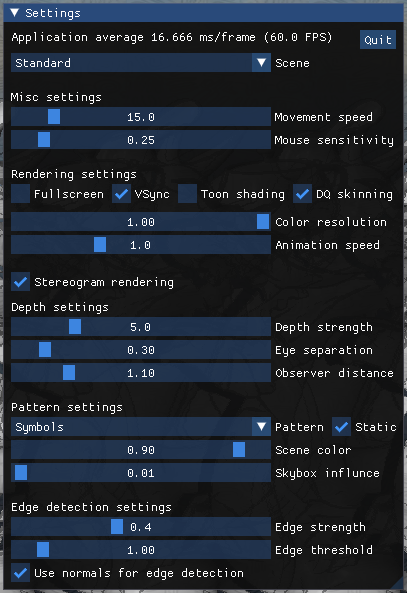
\includegraphics[width=0.6\textwidth]{img/gui.png}
    \captionof{figure}{Settings GUI}
\end{center}
The variables affected by the GUI are placed in a struct \textbf{Context} that is created in the \textbf{main} and
passed as a pointer to most objects in the application. This avoids proliferation of global variables for data 
that need to be shader by multiple objects.

\section{Classical rendering}
\subsection{Rendering class}
The \textbf{Render} class is responsible for setting up the general rendering state, such as back face culling, creating
the FBO, keeping them of the correct size when the window resize and calculate the delta time.\\\\
The \textbf{Render} holds the objects responsible for each render pass and call them in the correct order on the appropriate
framebuffer.
\begin{lstlisting}[caption={Main rendering loop},captionpos=b]
// Illumination pass
glViewport(0, 0, ctx->width, ctx->height);
glBindFramebuffer(GL_FRAMEBUFFER, ctx->stereoRendering ? FBO:0);
glClear(GL_COLOR_BUFFER_BIT | GL_DEPTH_BUFFER_BIT);

GLenum buffers[] = {GL_COLOR_ATTACHMENT0, GL_COLOR_ATTACHMENT1};
glDrawBuffers(2, buffers);
illumPass.execute(scene);

// SkyboxPass
skyboxPass.execute(scene, ctx);

// Stereogram pass
glDrawBuffers(1, buffers);
if (ctx->stereoRendering) {
    glBindFramebuffer(GL_FRAMEBUFFER, 0);
    stereoPass.execute(color, depth, normal);
}

// UI
if (ctx->showMenu) {
    gui.RenderMenu();
}

// Swap buffer
glfwSwapBuffers(window);
glfwSwapInterval(ctx->vSync);
\end{lstlisting}
\subsection{Illumination pass}
The illumination pass set up the view and projection matrix based as provided by the \textbf{SceneCamera} and then iterate
every object in the scene setting up its model matrix, its material uniform, binding its texture and drawing its model.\\\\
The illumination model is Blinn-Phong, as object blends one over each other more sophisticated illumination model give little
visible difference and so a simple and fast model was preferred for this project.\\\\
A different subroutine can be called to apply toon shading. This simply use \textbf{step} to quantize the illumination.
\begin{lstlisting}[caption={Toon shading subroutine version},captionpos=b]
[...]
float lambertian = step(0.5, max(dot(lightDir, normal), 0.0));
[...]
float specular = step(0.2, pow(specAngle, shininess));
[...]
\end{lstlisting}
\begin{center}
    \centering
    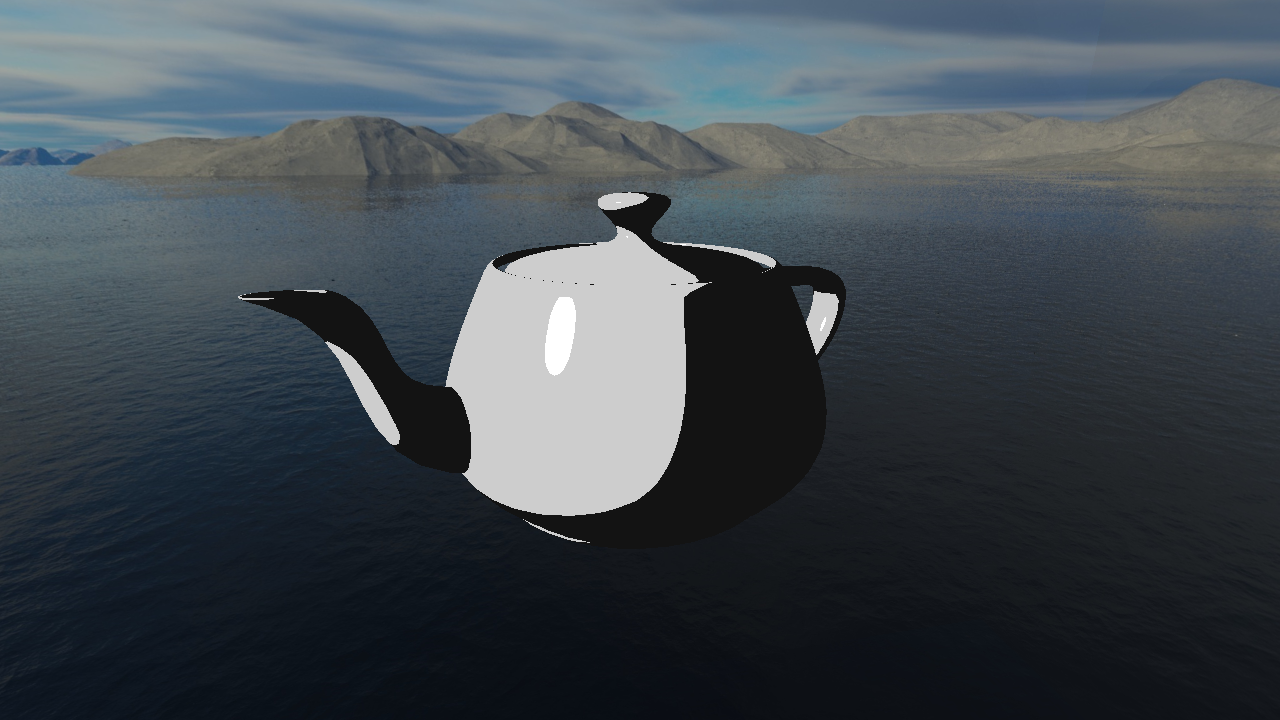
\includegraphics[width=1.0\textwidth]{img/toon.png}
    \captionof{figure}{Toon shaded teapot}
\end{center}
It is also possible to quantize the color resolution to apply a more cartoonish effect. This can create a lot
of banding. The result, once the pixel are blended over each other for the stereogram rendering, is still quite nice.\\\\
During this pass we also save the view space normal on a texture, they will be used for edge detection in the stereogram
rendering pass.

\subsection{Skybox pass}
The skybox pass draws the skybox after all the other models were drawn to avoid processing fragment that will belong to an object
in the scene.\\\\
The only difference from a standard skybox rendering is that the alpha component of the fragment is set based
on the GUI setting \textbf{Skybox influence}. This does not affect the rendering color, as alpha blending is not enabled, but
is used for the stereogram pass to achieve some advanced effects.

\section{Autostereogram rendering}
\subsection{Main algorithm}
The autostereogram rendering is executed in 2 passes each one rendering a fullscreen quad.\\\\
In the first pass we sample the depth buffer from the current texel moving to the left border to link
all the texel that will need to have the same color in the final rendering.
\begin{lstlisting}[caption={Autostereogram depth sampling},captionpos=b]
vec2 currCoord = uv;
for(int i = 0; i < 32; i++) {
    float depth = sampleDepth(currCoord);
    float sep = eyeSep*depth/(depth + obsDistance);
    if(currCoord.x < 0.0)
       break;
    currCoord.x -= sep;
}
currCoord.x = mod(currCoord.x, 1.0);
\end{lstlisting}
Using this method we simply need to assign the same color to each texel having the same \textbf{currCoord}.\\\\
The depth sample from the depth buffer is not linear and should be linearized to have the correct results.
Sadly autostereogram can provide only a limited range of depth, linearizing this would require to clamp the max depth
to a really close value. To allow some perception of the depth difference of far away object it was preferred to not linearize
the depth making close object more visibly 3D while keeping some little 3D effect for far away one. This can be also made even less linear
as the depth value get changed using an exponential function having as the exponent be GUI setting \textbf{depth strength}. Note that value too high
cause glitches to close object, while low values reduce the 3D effect.\\\\
To allow the scene color to be used we also store the current texel color in a SSBO as we will discuss later, for this
reason a second pass is required after a barrier to ensure all data written to the SSBO will be read correctly in the second pass.\\\\
The value of \textbf{currCoord} will be also needed in the second pass, to avoid computing it again we store it in another SSBO.\\\\
We also detect if the current texel is a edge and store this information in the 3rd and last SSBO, we will better discuss this later.

\subsection{Pattern}
In the second pass we assign the texel color sampling a pattern based on the value of \textbf{currCoord}.\\\\
The application support random generated patter with perlin noise, either RGB or grayscale. The perlin noise
can also take into account the current frame time to make it animated.\\\\
Another option that avoid the expensive perlin noise generation is to sample a texture. To animate the texture pattern
we just move the UV coordinate a bit each frame.\\\\
The last option is to use an animated texture pattern, in this case for simplicity all frame was placed in a single texture
and the code sample in the correct position based on the current time. As a pattern texture is only 256x256 pixel having
64 frames in a texture only requires a 2048x2048 texture that is totally manageable by the GPU.

\subsection{Scene color}
During the first pass we save the texel color in a SSBO. As many texel will have the same \textbf{currCoord} we will
need to blend them together and use the average as the final color. This scene color can then be mixed with the color
generated from the pattern.\\\\
To average the color, in the first pass, we atomically add each color in the SSBO using the alpha channel as a counter of how many texel
were added for that value of \textbf{currCoord}. In the second pass we simply divide the RGB channels by the alpha to get the correct values back.
Note that is possible to do atomic operation only on integer scalar values.
\begin{lstlisting}[caption={First pass color blending},captionpos=b]
UV[index(uv)] = currCoord;
vec4 col = texture(colorTex, uv);
col.rgb *= col.a;
int i = index(currCoord);
atomicAdd(color[i].r, int(col.r*4096));
atomicAdd(color[i].g, int(col.g*4096));
atomicAdd(color[i].b, int(col.b*4096));
atomicAdd(color[i].a, int(col.a*4096));
\end{lstlisting}

\begin{lstlisting}[caption={Second pass color blending},captionpos=b]
vec2 co = UV[index(uv)];
int i = index(co);
vec3 random = pattern(co);
vec3 col = vec3(0.0);
if (color[i].w != 0) {
    col = color[i].rgb/float(color[i].w);
}
\end{lstlisting}
In the previous code \textbf{index} is a helper function to get the 1D array index from 2D coordinates.\\\\
It is also possible to use this alpha as a weight to give different importance to some object in the scene. For example the skybox might have a low weight
making it bleed over other pixel only if there was no other important object that should bleed over that pixel.
To have alpha value greater than 1 the FBO color attachment texture should be declared using a not clamped format such as GL\_RGBA32F.
\begin{center}
    \centering
    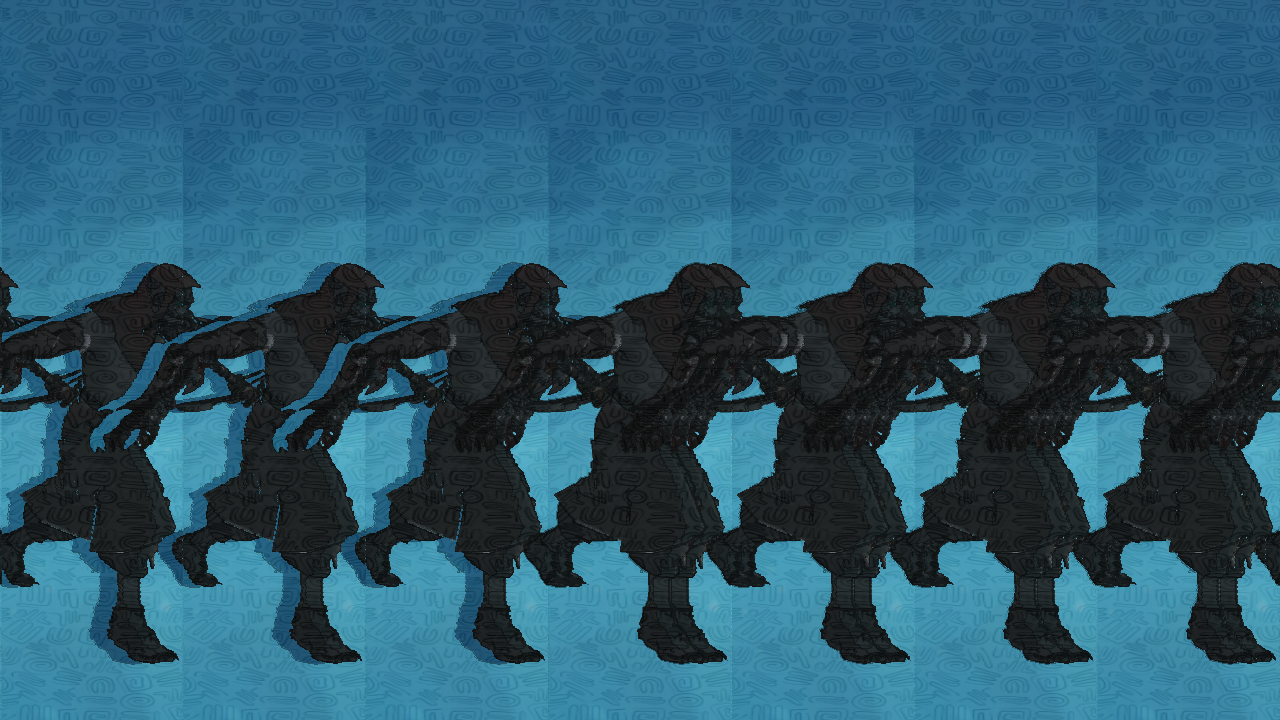
\includegraphics[width=1.0\textwidth]{img/dance.png}
    \captionof{figure}{Dancer autostereogram}
\end{center}
Here we can see how the blue of the skybox does not blend with the colors of the dancing goblin as it have a weight of 0.01 as compared to the
1.0 of the dancer.

\subsection{Edge detection}
To enchant the autostereogram sharpness we can add the object edged to the image.\\\\
In the first pass we detect the edge using Sobel either on the scene color or on the scene view space normals. The second case give better results 
but is unable to detect edges in the object texture.\\\\
Once we have detected the edge we store this information in a SSBO. In the second pass we check if there was an edge in any texel having
that particular \textbf{currCoord}, if it is the case we render a darker color.
\begin{center}
    \centering
    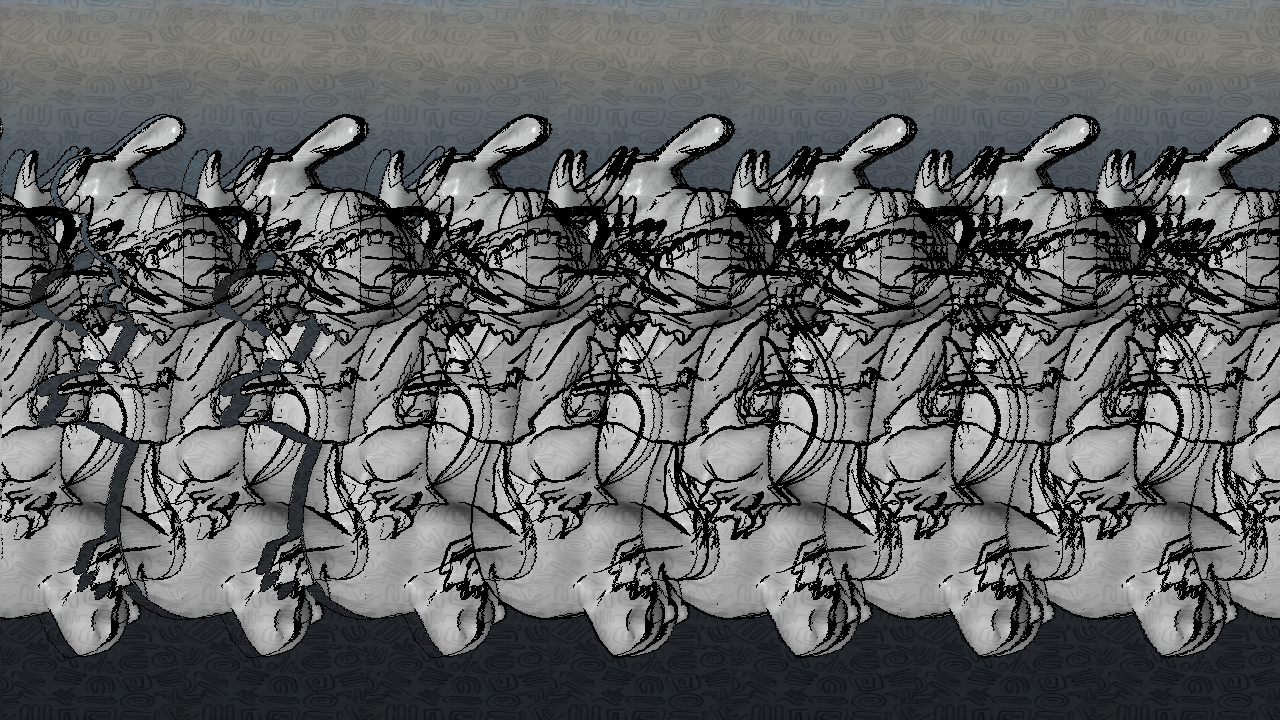
\includegraphics[width=1.0\textwidth]{img/edge.png}
    \captionof{figure}{Edge detection on normals}
\end{center}

\subsection{Numerical errors}
Numerical precision can lead to graphical artefacts.
\begin{center}
    \centering
    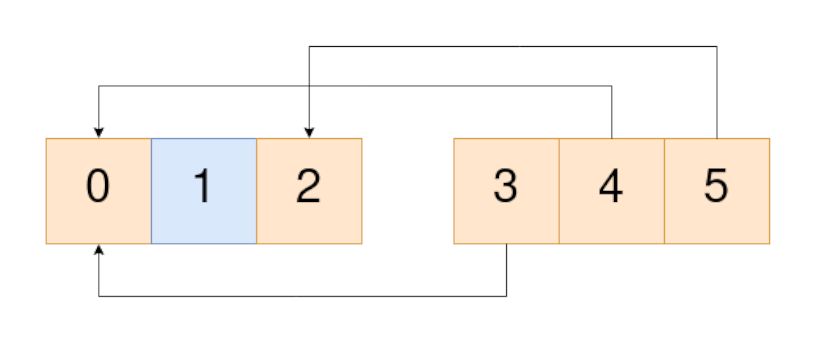
\includegraphics[width=1.0\textwidth]{img/pixel.png}
    \captionof{figure}{Numerical error cause wrong pixel colors}
\end{center}
In this example the pixel 0, 1 and 2 belong to the skybox, when
the pixel 3, 4 and 5 belonging to an object blend with them, due little numerical
errors the pixel 4 calculate its \textbf{currCoord} to be the same as pixel 0 rather
than pixel 1. As a result the pixel 1 will keep the skybox color causing a visible
wrongly colored pixel.

\begin{center}
    \centering
    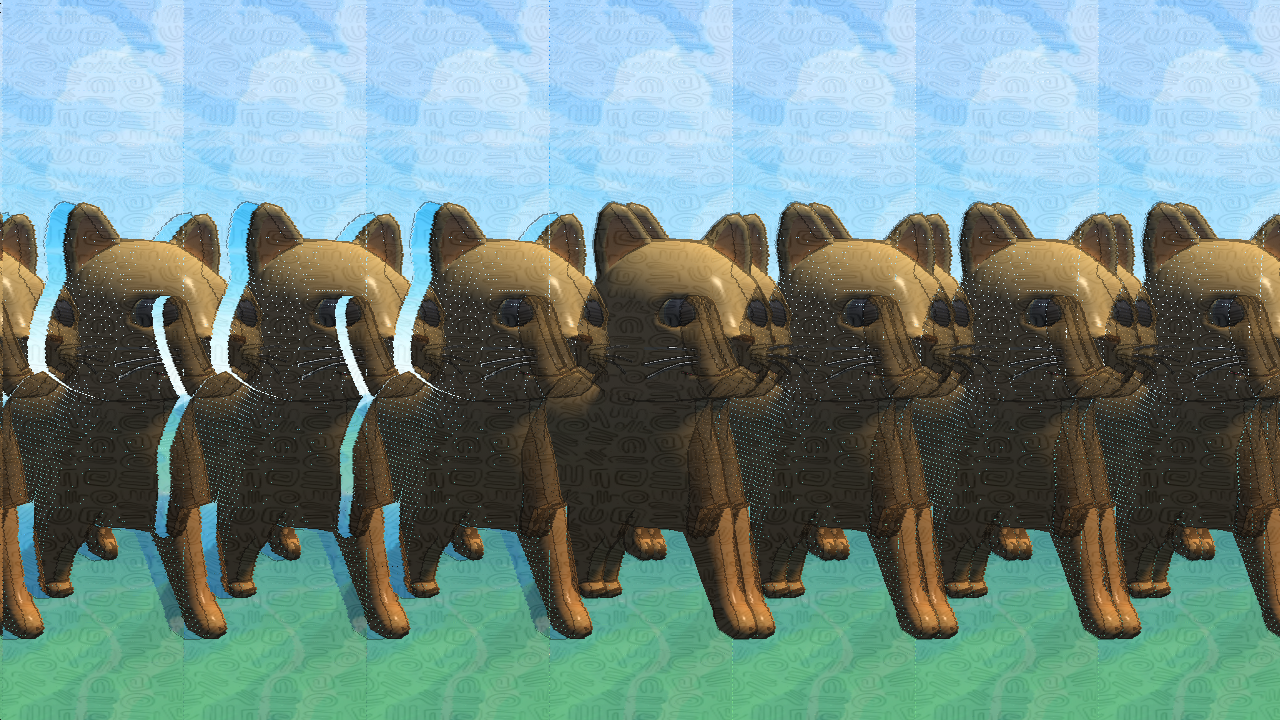
\includegraphics[width=1.0\textwidth]{img/error.png}
    \captionof{figure}{Numerical error artefact}
\end{center}

This problem looks like a salt and pepper noise, so we can use a median filter to mitigate it. For each texel
we sample also the 2 texels above and below and the 2 texels on the side. We then sort the 5 texel values and take
the median one.

\begin{center}
    \centering
    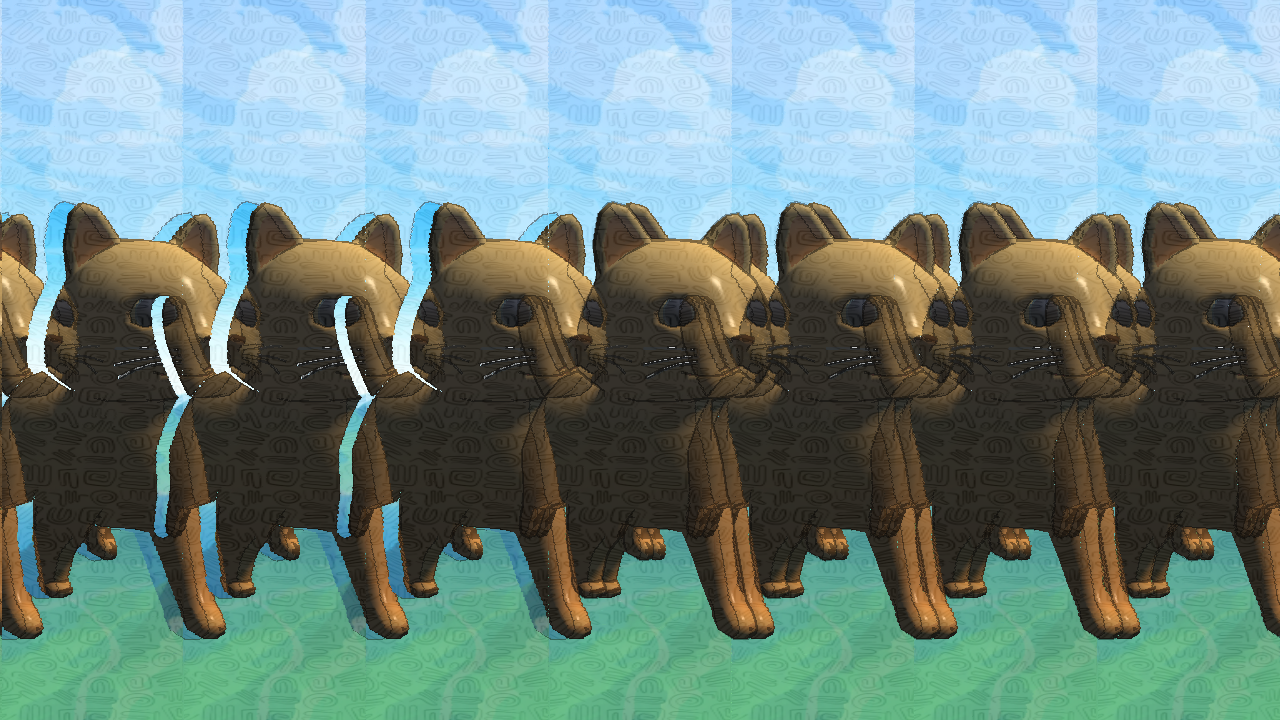
\includegraphics[width=1.0\textwidth]{img/fix.png}
    \captionof{figure}{Median filtering result}
\end{center}
The result is not perfected but greatly improved, mixing with the pattern also help to hide the artefacts.

\section{Skeletal animation}

\subsection{Linear blend skinning}
Linear blend skinning code was based on Learn OpenGL implementation. The animation is loaded from the mesh file using assimp.
At each frame we compute the current bone trasformations interpolating between keyframes. To get the correct results rotation
need to be interpolated using quaternions. The final trasform for each bone is then computed comulating each bone trasform with the base
trasform of each bone. The final transforms are sent to the GPU as uniform for the vertex shader.\\\\
To achieve better results blend skinning is used. Each vertex is associated with up to 4 bone
of the skeleton. For each of these bone there is a weight that encode how much the vertex is affected by that bone.
In the vertex shader we interpolate the bone final transforms with the weights and then apply the result to the vertex to get
the vertex position in object space.\\\\
With linear blend skinning we represent the trasformations as matrices and we interpolate linearly between them.
This approach mostly work, but does not preserve the mesh volume and can lead to some artefacts such as candy wrap.

\subsection{Dual quaternion skinning}
An alternative approach that preserve the volumes is dual quaternion skinning. For this we represent the bone final trasformations as dual quaternion
and interpolate between them.\\\\
Note that dual quaternions can only encode rototraslations and scaling need to be interpolated on his own. While most animation have no need for scaling
it seem that most animation loaded from various assets have a constant scaling applied to bones.\\\\
A dual quaternion is a number in the form:
\[
    p + \epsilon q \text{ where } p, q \in \mathbb{H}\\\\
    \epsilon \neq 0, \epsilon^2 = 0
\]
A rototraslations is expressed as a unitary dual quaternion:
\[
    \|p + \epsilon q\| = 1 \iff \|p\| = 1 \land p \cdot q = 0
\]
A rotation around an axis $(x, y, z)$ of an angle $\theta$ is expressed as with normal quaternions:
\[
    \cos(\frac{\theta}{2})+\sin(\frac{\theta}{2})(xi + yj + zk)
\]
A translation $(x, y, z)$ is expressed as:
\[
    1+\frac{\epsilon}{2}(xi + yj + zk)
\]
A point $(x, y, z) \in \mathbb{E}^3$ is expressed as a dual quaternion like this:
\[
    1 + \epsilon xi + \epsilon yj + \epsilon zk
\]
To apply a rototraslation expressed by $t$ to the point $a$:
\[
    a' = ta\overline{t} \text{ where } \overline{p + \epsilon q} = \overline{p} - \epsilon \overline{q}
\]
To obtain the rotation and the translation expressed by the final transform matrix the method \textbf{glm::decompose} was used.
The dual quaternion is then computed and sent to the GPU as uniform.\\\\
In the shader we interpolate the dual quaternion linearly (taking into account the shortest path), normalize the result and then apply the it to the vertex position.
To normalize a dual quaternion we first divide both $p$ and $q$ by $\|p\|$ and then subtract from $q$ the value of $(p \cdot q)p$.
\begin{center}
    \centering
    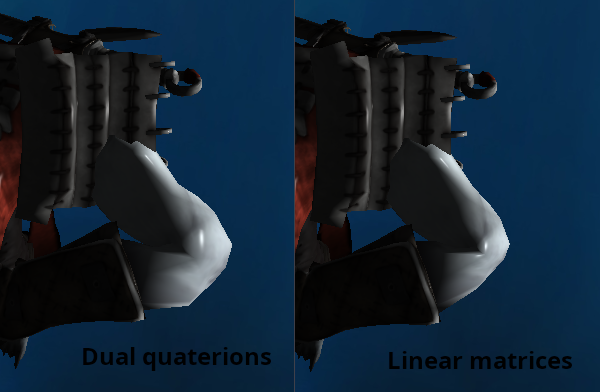
\includegraphics[width=0.8\textwidth]{img/dq.png}
    \captionof{figure}{Dual quaternions skinning comparation}
\end{center}
To calculate the vertex normal we usually need the inverse of the transpose of the transformation matrix. As dual quaternions only encode rototranslation
we can apply the dual quaternion as it is.

\section{Performance evaluation}

\section{Conclusion}

\end{document}